% Options for packages loaded elsewhere
\PassOptionsToPackage{unicode}{hyperref}
\PassOptionsToPackage{hyphens}{url}
\documentclass[
  11pt,
]{article}
\usepackage{xcolor}
\usepackage[margin=1in]{geometry}
\usepackage{amsmath,amssymb}
\setcounter{secnumdepth}{5}
\usepackage{iftex}
\ifPDFTeX
  \usepackage[T1]{fontenc}
  \usepackage[utf8]{inputenc}
  \usepackage{textcomp} % provide euro and other symbols
\else % if luatex or xetex
  \usepackage{unicode-math} % this also loads fontspec
  \defaultfontfeatures{Scale=MatchLowercase}
  \defaultfontfeatures[\rmfamily]{Ligatures=TeX,Scale=1}
\fi
\usepackage{lmodern}
\ifPDFTeX\else
  % xetex/luatex font selection
\fi
% Use upquote if available, for straight quotes in verbatim environments
\IfFileExists{upquote.sty}{\usepackage{upquote}}{}
\IfFileExists{microtype.sty}{% use microtype if available
  \usepackage[]{microtype}
  \UseMicrotypeSet[protrusion]{basicmath} % disable protrusion for tt fonts
}{}
\makeatletter
\@ifundefined{KOMAClassName}{% if non-KOMA class
  \IfFileExists{parskip.sty}{%
    \usepackage{parskip}
  }{% else
    \setlength{\parindent}{0pt}
    \setlength{\parskip}{6pt plus 2pt minus 1pt}}
}{% if KOMA class
  \KOMAoptions{parskip=half}}
\makeatother
\usepackage{color}
\usepackage{fancyvrb}
\newcommand{\VerbBar}{|}
\newcommand{\VERB}{\Verb[commandchars=\\\{\}]}
\DefineVerbatimEnvironment{Highlighting}{Verbatim}{commandchars=\\\{\}}
% Add ',fontsize=\small' for more characters per line
\usepackage{framed}
\definecolor{shadecolor}{RGB}{248,248,248}
\newenvironment{Shaded}{\begin{snugshade}}{\end{snugshade}}
\newcommand{\AlertTok}[1]{\textcolor[rgb]{0.94,0.16,0.16}{#1}}
\newcommand{\AnnotationTok}[1]{\textcolor[rgb]{0.56,0.35,0.01}{\textbf{\textit{#1}}}}
\newcommand{\AttributeTok}[1]{\textcolor[rgb]{0.13,0.29,0.53}{#1}}
\newcommand{\BaseNTok}[1]{\textcolor[rgb]{0.00,0.00,0.81}{#1}}
\newcommand{\BuiltInTok}[1]{#1}
\newcommand{\CharTok}[1]{\textcolor[rgb]{0.31,0.60,0.02}{#1}}
\newcommand{\CommentTok}[1]{\textcolor[rgb]{0.56,0.35,0.01}{\textit{#1}}}
\newcommand{\CommentVarTok}[1]{\textcolor[rgb]{0.56,0.35,0.01}{\textbf{\textit{#1}}}}
\newcommand{\ConstantTok}[1]{\textcolor[rgb]{0.56,0.35,0.01}{#1}}
\newcommand{\ControlFlowTok}[1]{\textcolor[rgb]{0.13,0.29,0.53}{\textbf{#1}}}
\newcommand{\DataTypeTok}[1]{\textcolor[rgb]{0.13,0.29,0.53}{#1}}
\newcommand{\DecValTok}[1]{\textcolor[rgb]{0.00,0.00,0.81}{#1}}
\newcommand{\DocumentationTok}[1]{\textcolor[rgb]{0.56,0.35,0.01}{\textbf{\textit{#1}}}}
\newcommand{\ErrorTok}[1]{\textcolor[rgb]{0.64,0.00,0.00}{\textbf{#1}}}
\newcommand{\ExtensionTok}[1]{#1}
\newcommand{\FloatTok}[1]{\textcolor[rgb]{0.00,0.00,0.81}{#1}}
\newcommand{\FunctionTok}[1]{\textcolor[rgb]{0.13,0.29,0.53}{\textbf{#1}}}
\newcommand{\ImportTok}[1]{#1}
\newcommand{\InformationTok}[1]{\textcolor[rgb]{0.56,0.35,0.01}{\textbf{\textit{#1}}}}
\newcommand{\KeywordTok}[1]{\textcolor[rgb]{0.13,0.29,0.53}{\textbf{#1}}}
\newcommand{\NormalTok}[1]{#1}
\newcommand{\OperatorTok}[1]{\textcolor[rgb]{0.81,0.36,0.00}{\textbf{#1}}}
\newcommand{\OtherTok}[1]{\textcolor[rgb]{0.56,0.35,0.01}{#1}}
\newcommand{\PreprocessorTok}[1]{\textcolor[rgb]{0.56,0.35,0.01}{\textit{#1}}}
\newcommand{\RegionMarkerTok}[1]{#1}
\newcommand{\SpecialCharTok}[1]{\textcolor[rgb]{0.81,0.36,0.00}{\textbf{#1}}}
\newcommand{\SpecialStringTok}[1]{\textcolor[rgb]{0.31,0.60,0.02}{#1}}
\newcommand{\StringTok}[1]{\textcolor[rgb]{0.31,0.60,0.02}{#1}}
\newcommand{\VariableTok}[1]{\textcolor[rgb]{0.00,0.00,0.00}{#1}}
\newcommand{\VerbatimStringTok}[1]{\textcolor[rgb]{0.31,0.60,0.02}{#1}}
\newcommand{\WarningTok}[1]{\textcolor[rgb]{0.56,0.35,0.01}{\textbf{\textit{#1}}}}
\usepackage{graphicx}
\makeatletter
\newsavebox\pandoc@box
\newcommand*\pandocbounded[1]{% scales image to fit in text height/width
  \sbox\pandoc@box{#1}%
  \Gscale@div\@tempa{\textheight}{\dimexpr\ht\pandoc@box+\dp\pandoc@box\relax}%
  \Gscale@div\@tempb{\linewidth}{\wd\pandoc@box}%
  \ifdim\@tempb\p@<\@tempa\p@\let\@tempa\@tempb\fi% select the smaller of both
  \ifdim\@tempa\p@<\p@\scalebox{\@tempa}{\usebox\pandoc@box}%
  \else\usebox{\pandoc@box}%
  \fi%
}
% Set default figure placement to htbp
\def\fps@figure{htbp}
\makeatother
\setlength{\emergencystretch}{3em} % prevent overfull lines
\providecommand{\tightlist}{%
  \setlength{\itemsep}{0pt}\setlength{\parskip}{0pt}}
\usepackage{amsmath}
% Shared LaTeX preamble for all Data Mining / ISLR chapter documents.
% Provides \makecoverpage{<assignment title>} — a standalone title page
% with fixed student identity, so every chapter/lab looks uniform.

\usepackage{graphicx}

\newcommand{\makecoverpage}[1]{%
\begin{titlepage}
\centering
\vspace*{2cm}

{\Large \textbf{Adventist University of Central Africa}}\\[0.4cm]
{\large Master's in Big Data Analytics}\\[2cm]

{\Huge \textbf{#1}}\\[0.5cm]
{\large \textit{Introduction to Statistical Learning with Applications in R}}\\[3cm]

\begin{tabular}{rl}
\textbf{Programme:} & MSc Big Data Analytics \\
\textbf{Course Title:} & Data Mining \\
\textbf{Course Code:} & MSDA 9124 \\
\textbf{Lecturer:} & Dr. Pacifique Nizeyimana \\
\textbf{Student Name:} & Wayne Rubangisa \\
\textbf{Student ID:} & 101220 \\
\end{tabular}

\vfill

{\large September 2026}

\end{titlepage}
}

\usepackage{bookmark}
\IfFileExists{xurl.sty}{\usepackage{xurl}}{} % add URL line breaks if available
\urlstyle{same}
\hypersetup{
  hidelinks,
  pdfcreator={LaTeX via pandoc}}

\author{}
\date{\vspace{-2.5em}}

\begin{document}

\makecoverpage{Chapter 4 --- Classification \\ Exercises 5, 10, 14, and 16}

\begin{Shaded}
\begin{Highlighting}[]
\FunctionTok{library}\NormalTok{(ISLR2)}
\FunctionTok{library}\NormalTok{(MASS)}
\FunctionTok{library}\NormalTok{(class)}
\FunctionTok{library}\NormalTok{(e1071)}
\end{Highlighting}
\end{Shaded}

Note: this document loads both \texttt{ISLR2} and \texttt{MASS}, and
both packages export a data set called \texttt{Boston}
(\texttt{MASS::Boston} has 14 columns, including a variable dropped from
\texttt{ISLR2::Boston}'s 13). Because \texttt{MASS} is attached after
\texttt{ISLR2}, it sits earlier on R's search path --- so an unqualified
\texttt{Boston} would silently resolve to \texttt{MASS::Boston}, not the
one the book actually uses. Exercise 16 below refers to it explicitly as
\texttt{ISLR2::Boston} throughout to avoid that trap.

\section{Exercise 5 --- LDA vs.~QDA}\label{exercise-5-lda-vs.-qda}

\subsection{(a) Bayes boundary is
linear}\label{a-bayes-boundary-is-linear}

\textbf{Training set:} QDA will (weakly) achieve better training
performance --- it has strictly more flexibility, so it can always fit
the training data at least as well as LDA, and typically better, by
using its extra covariance parameters to bend the boundary even when it
doesn't need to.

\textbf{Test set:} LDA should perform better. If the true Bayes boundary
really is linear, LDA's assumption matches reality exactly, while QDA is
estimating a more flexible boundary than the data actually calls for.
That extra flexibility doesn't reduce bias here (there's no bias to
reduce --- LDA is already unbiased for a linear boundary), so it's pure
added variance from estimating a much larger number of covariance
parameters, which typically shows up as worse test performance.

\subsection{(b) Bayes boundary is
non-linear}\label{b-bayes-boundary-is-non-linear}

\textbf{Training set:} QDA again fits at least as well, for the same
reason as (a).

\textbf{Test set:} QDA should perform better. Now LDA's linear
assumption is genuinely wrong, so it carries irreducible bias no amount
of data can fix. QDA can actually approximate the curvature, trading
some added variance for a real reduction in bias --- and as long as
there's enough data to estimate the extra parameters reasonably well,
that trade tends to pay off.

\subsection{\texorpdfstring{(c) As \(n\)
increases}{(c) As n increases}}\label{c-as-n-increases}

We'd expect QDA's relative test accuracy to \textbf{improve}. QDA has
more parameters to estimate (a full covariance matrix per class, rather
than one shared matrix), so its variance is more sensitive to sample
size. With more data, QDA's parameter estimates get more stable ---
closing the variance gap with LDA --- while gaining nothing changes for
LDA's bias if the truth isn't linear. So more data specifically helps
the model that needed it most.

\subsection{(d) True or False: QDA is superior even when the Bayes
boundary is linear, because it's flexible enough to approximate a linear
boundary}\label{d-true-or-false-qda-is-superior-even-when-the-bayes-boundary-is-linear-because-its-flexible-enough-to-approximate-a-linear-boundary}

\textbf{False.} This is exactly the setup from part (a). Yes, QDA is
flexible enough to approximate a linear boundary reasonably closely ---
but ``flexible enough to approximate it'' is not the same as ``better at
estimating it.'' QDA has to \emph{estimate} that near-linear shape from
finite, noisy data using far more parameters than LDA needs, and that
estimation variance is real cost with no offsetting benefit, since LDA
already targets the right boundary shape exactly. The claim mistakes
flexibility for accuracy --- more flexibility only helps when the extra
bias reduction it buys outweighs the extra variance it costs, and here
there's no bias to reduce in the first place.

\newpage

\section{\texorpdfstring{Exercise 10 --- The LDA Log-Odds Formula for
\(p = 1\)}{Exercise 10 --- The LDA Log-Odds Formula for p = 1}}\label{exercise-10-the-lda-log-odds-formula-for-p-1}

The general (\(p > 1\)) result gives the log-odds between class \(k\)
and a baseline class \(K\) as a linear function of \(x\):

\[
\log\left(\frac{\Pr(Y=k \mid X=x)}{\Pr(Y=K \mid X=x)}\right) = a_k + \sum_{j=1}^p b_{kj} x_j
\]

with \(a_k\) and \(b_{kj}\) expressed in terms of the class priors
\(\pi_k\), class mean vectors \(\mu_k\), and the shared covariance
matrix \(\Sigma\). For \(p=1\), every one of those quantities collapses
to a scalar: \(\mu_k\) becomes a single number, and \(\Sigma\) becomes
the shared variance \(\sigma^2\).

Under LDA's assumptions, \(X \mid Y=k \sim N(\mu_k, \sigma^2)\), so the
one-dimensional normal density is

\[
f_k(x) = \frac{1}{\sqrt{2\pi}\,\sigma} \exp\left(-\frac{(x-\mu_k)^2}{2\sigma^2}\right)
\]

By Bayes' theorem, \(\Pr(Y=k\mid X=x) \propto \pi_k f_k(x)\), so the
log-odds between class \(k\) and class \(K\) is

\[
\log\left(\frac{\Pr(Y=k\mid X=x)}{\Pr(Y=K\mid X=x)}\right)
= \log\left(\frac{\pi_k f_k(x)}{\pi_K f_K(x)}\right)
= \log\left(\frac{\pi_k}{\pi_K}\right) + \log\left(\frac{f_k(x)}{f_K(x)}\right)
\]

The \(\frac{1}{\sqrt{2\pi}\sigma}\) normalizing constants are identical
for every class (shared \(\sigma^2\)), so they cancel in the ratio
\(f_k(x)/f_K(x)\), leaving

\[
\log\left(\frac{f_k(x)}{f_K(x)}\right)
= -\frac{(x-\mu_k)^2}{2\sigma^2} + \frac{(x-\mu_K)^2}{2\sigma^2}
= \frac{1}{2\sigma^2}\Big[(x-\mu_K)^2 - (x-\mu_k)^2\Big]
\]

Expanding both squares --- \((x-\mu_K)^2 = x^2 - 2x\mu_K + \mu_K^2\) and
similarly for \(\mu_k\) --- the \(x^2\) terms cancel between them,
leaving only terms linear in \(x\) plus constants:

\[
(x-\mu_K)^2 - (x-\mu_k)^2 = 2x(\mu_k - \mu_K) - (\mu_k^2 - \mu_K^2)
\]

Putting it all together:

\[
\log\left(\frac{\Pr(Y=k\mid X=x)}{\Pr(Y=K\mid X=x)}\right)
= \underbrace{\log\left(\frac{\pi_k}{\pi_K}\right) - \frac{\mu_k^2 - \mu_K^2}{2\sigma^2}}_{a_k}
\; + \; \underbrace{\frac{\mu_k - \mu_K}{\sigma^2}}_{b_{k1}} \cdot x
\]

so, matching the target form (with the single predictor playing the role
of \(x_1\), i.e.~\(j=1\)):

\[
a_k = \log\left(\frac{\pi_k}{\pi_K}\right) - \frac{\mu_k^2 - \mu_K^2}{2\sigma^2},
\qquad
b_{k1} = \frac{\mu_k - \mu_K}{\sigma^2}
\]

This is exactly the general \(p\)-dimensional result specialized to a
single feature: \(a_k\) still combines the log prior-odds with a term
penalizing classes whose mean is far from the origin (relative to their
shared variance), and \(b_{k1}\) is still \(\Sigma^{-1}(\mu_k - \mu_K)\)
--- just with matrix inversion trivialized to ordinary division by the
scalar \(\sigma^2\).

\newpage

\section{\texorpdfstring{Exercise 14 --- Predicting High/Low
\texttt{mpg} for the \texttt{Auto}
Data}{Exercise 14 --- Predicting High/Low mpg for the Auto Data}}\label{exercise-14-predicting-highlow-mpg-for-the-auto-data}

\subsection{\texorpdfstring{(a) Creating
\texttt{mpg01}}{(a) Creating mpg01}}\label{a-creating-mpg01}

\begin{Shaded}
\begin{Highlighting}[]
\NormalTok{Auto2 }\OtherTok{\textless{}{-}}\NormalTok{ Auto}
\NormalTok{Auto2}\SpecialCharTok{$}\NormalTok{mpg01 }\OtherTok{\textless{}{-}} \FunctionTok{as.integer}\NormalTok{(Auto2}\SpecialCharTok{$}\NormalTok{mpg }\SpecialCharTok{\textgreater{}} \FunctionTok{median}\NormalTok{(Auto2}\SpecialCharTok{$}\NormalTok{mpg))}
\FunctionTok{table}\NormalTok{(Auto2}\SpecialCharTok{$}\NormalTok{mpg01)}
\end{Highlighting}
\end{Shaded}

\begin{verbatim}
## 
##   0   1 
## 196 196
\end{verbatim}

Splitting exactly at the median naturally gives a near-perfectly
balanced binary outcome (196/196) --- useful, since classification
methods generally work best when neither class dominates.

\subsection{\texorpdfstring{(b) Exploring associations with
\texttt{mpg01}}{(b) Exploring associations with mpg01}}\label{b-exploring-associations-with-mpg01}

\begin{Shaded}
\begin{Highlighting}[]
\FunctionTok{par}\NormalTok{(}\AttributeTok{mfrow =} \FunctionTok{c}\NormalTok{(}\DecValTok{2}\NormalTok{, }\DecValTok{2}\NormalTok{))}
\FunctionTok{boxplot}\NormalTok{(weight }\SpecialCharTok{\textasciitilde{}}\NormalTok{ mpg01, }\AttributeTok{data =}\NormalTok{ Auto2, }\AttributeTok{main =} \StringTok{"Weight vs mpg01"}\NormalTok{,}
        \AttributeTok{xlab =} \StringTok{"mpg01"}\NormalTok{, }\AttributeTok{ylab =} \StringTok{"weight"}\NormalTok{)}
\FunctionTok{boxplot}\NormalTok{(displacement }\SpecialCharTok{\textasciitilde{}}\NormalTok{ mpg01, }\AttributeTok{data =}\NormalTok{ Auto2, }\AttributeTok{main =} \StringTok{"Displacement vs mpg01"}\NormalTok{,}
        \AttributeTok{xlab =} \StringTok{"mpg01"}\NormalTok{, }\AttributeTok{ylab =} \StringTok{"displacement"}\NormalTok{)}
\FunctionTok{boxplot}\NormalTok{(horsepower }\SpecialCharTok{\textasciitilde{}}\NormalTok{ mpg01, }\AttributeTok{data =}\NormalTok{ Auto2, }\AttributeTok{main =} \StringTok{"Horsepower vs mpg01"}\NormalTok{,}
        \AttributeTok{xlab =} \StringTok{"mpg01"}\NormalTok{, }\AttributeTok{ylab =} \StringTok{"horsepower"}\NormalTok{)}
\FunctionTok{boxplot}\NormalTok{(cylinders }\SpecialCharTok{\textasciitilde{}}\NormalTok{ mpg01, }\AttributeTok{data =}\NormalTok{ Auto2, }\AttributeTok{main =} \StringTok{"Cylinders vs mpg01"}\NormalTok{,}
        \AttributeTok{xlab =} \StringTok{"mpg01"}\NormalTok{, }\AttributeTok{ylab =} \StringTok{"cylinders"}\NormalTok{)}
\end{Highlighting}
\end{Shaded}

\begin{center}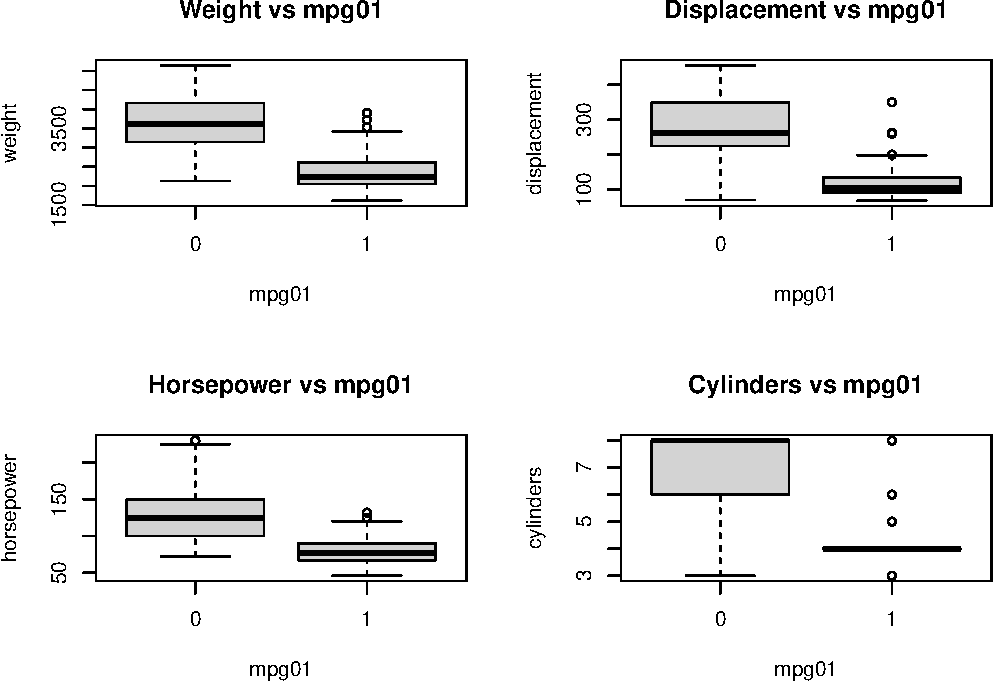
\includegraphics{ch04_exercises_files/figure-latex/mpg01-explore-1} \end{center}

\begin{Shaded}
\begin{Highlighting}[]
\FunctionTok{sort}\NormalTok{(}\FunctionTok{abs}\NormalTok{(}\FunctionTok{sapply}\NormalTok{(Auto2[, }\FunctionTok{c}\NormalTok{(}\StringTok{"cylinders"}\NormalTok{,}\StringTok{"displacement"}\NormalTok{,}\StringTok{"horsepower"}\NormalTok{,}\StringTok{"weight"}\NormalTok{,}
                            \StringTok{"acceleration"}\NormalTok{,}\StringTok{"year"}\NormalTok{,}\StringTok{"origin"}\NormalTok{)],}
                 \ControlFlowTok{function}\NormalTok{(x) }\FunctionTok{cor}\NormalTok{(x, Auto2}\SpecialCharTok{$}\NormalTok{mpg01))), }\AttributeTok{decreasing =} \ConstantTok{TRUE}\NormalTok{)}
\end{Highlighting}
\end{Shaded}

\begin{verbatim}
##    cylinders       weight displacement   horsepower       origin         year 
##    0.7591939    0.7577566    0.7534766    0.6670526    0.5136984    0.4299042 
## acceleration 
##    0.3468215
\end{verbatim}

\texttt{weight}, \texttt{displacement}, \texttt{horsepower}, and
\texttt{cylinders} all separate the two \texttt{mpg01} groups cleanly in
the boxplots and are the four most correlated with \texttt{mpg01} (all
above 0.75 in magnitude) --- heavier, larger- engined, more-cylindered
cars cluster in the low-\texttt{mpg} group, which matches basic physical
intuition (more mass and engine displacement to move costs more fuel per
mile). These four are used as predictors below.

\subsection{(c) Train/test split}\label{c-traintest-split}

\begin{Shaded}
\begin{Highlighting}[]
\FunctionTok{set.seed}\NormalTok{(}\DecValTok{1}\NormalTok{)}
\NormalTok{n }\OtherTok{\textless{}{-}} \FunctionTok{nrow}\NormalTok{(Auto2)}
\NormalTok{train }\OtherTok{\textless{}{-}} \FunctionTok{sample}\NormalTok{(}\FunctionTok{seq\_len}\NormalTok{(n), }\AttributeTok{size =} \FunctionTok{floor}\NormalTok{(}\FloatTok{0.7} \SpecialCharTok{*}\NormalTok{ n))}
\NormalTok{train.set }\OtherTok{\textless{}{-}}\NormalTok{ Auto2[train, ]}
\NormalTok{test.set }\OtherTok{\textless{}{-}}\NormalTok{ Auto2[}\SpecialCharTok{{-}}\NormalTok{train, ]}

\NormalTok{vars }\OtherTok{\textless{}{-}} \FunctionTok{c}\NormalTok{(}\StringTok{"cylinders"}\NormalTok{, }\StringTok{"displacement"}\NormalTok{, }\StringTok{"horsepower"}\NormalTok{, }\StringTok{"weight"}\NormalTok{)}
\NormalTok{form }\OtherTok{\textless{}{-}} \FunctionTok{as.formula}\NormalTok{(}\FunctionTok{paste}\NormalTok{(}\StringTok{"mpg01 \textasciitilde{}"}\NormalTok{, }\FunctionTok{paste}\NormalTok{(vars, }\AttributeTok{collapse =} \StringTok{" + "}\NormalTok{)))}
\FunctionTok{c}\NormalTok{(}\AttributeTok{train =} \FunctionTok{nrow}\NormalTok{(train.set), }\AttributeTok{test =} \FunctionTok{nrow}\NormalTok{(test.set))}
\end{Highlighting}
\end{Shaded}

\begin{verbatim}
## train  test 
##   274   118
\end{verbatim}

\subsection{(d) LDA}\label{d-lda}

\begin{Shaded}
\begin{Highlighting}[]
\NormalTok{lda.fit }\OtherTok{\textless{}{-}} \FunctionTok{lda}\NormalTok{(form, }\AttributeTok{data =}\NormalTok{ train.set)}
\NormalTok{lda.pred }\OtherTok{\textless{}{-}} \FunctionTok{predict}\NormalTok{(lda.fit, test.set)}\SpecialCharTok{$}\NormalTok{class}
\NormalTok{lda.err }\OtherTok{\textless{}{-}} \FunctionTok{mean}\NormalTok{(lda.pred }\SpecialCharTok{!=}\NormalTok{ test.set}\SpecialCharTok{$}\NormalTok{mpg01)}
\NormalTok{lda.err}
\end{Highlighting}
\end{Shaded}

\begin{verbatim}
## [1] 0.1186441
\end{verbatim}

\subsection{(e) QDA}\label{e-qda}

\begin{Shaded}
\begin{Highlighting}[]
\NormalTok{qda.fit }\OtherTok{\textless{}{-}} \FunctionTok{qda}\NormalTok{(form, }\AttributeTok{data =}\NormalTok{ train.set)}
\NormalTok{qda.pred }\OtherTok{\textless{}{-}} \FunctionTok{predict}\NormalTok{(qda.fit, test.set)}\SpecialCharTok{$}\NormalTok{class}
\NormalTok{qda.err }\OtherTok{\textless{}{-}} \FunctionTok{mean}\NormalTok{(qda.pred }\SpecialCharTok{!=}\NormalTok{ test.set}\SpecialCharTok{$}\NormalTok{mpg01)}
\NormalTok{qda.err}
\end{Highlighting}
\end{Shaded}

\begin{verbatim}
## [1] 0.1186441
\end{verbatim}

\subsection{(f) Logistic regression}\label{f-logistic-regression}

\begin{Shaded}
\begin{Highlighting}[]
\NormalTok{glm.fit }\OtherTok{\textless{}{-}} \FunctionTok{glm}\NormalTok{(form, }\AttributeTok{data =}\NormalTok{ train.set, }\AttributeTok{family =}\NormalTok{ binomial)}
\NormalTok{glm.probs }\OtherTok{\textless{}{-}} \FunctionTok{predict}\NormalTok{(glm.fit, test.set, }\AttributeTok{type =} \StringTok{"response"}\NormalTok{)}
\NormalTok{glm.pred }\OtherTok{\textless{}{-}} \FunctionTok{ifelse}\NormalTok{(glm.probs }\SpecialCharTok{\textgreater{}} \FloatTok{0.5}\NormalTok{, }\DecValTok{1}\NormalTok{, }\DecValTok{0}\NormalTok{)}
\NormalTok{glm.err }\OtherTok{\textless{}{-}} \FunctionTok{mean}\NormalTok{(glm.pred }\SpecialCharTok{!=}\NormalTok{ test.set}\SpecialCharTok{$}\NormalTok{mpg01)}
\NormalTok{glm.err}
\end{Highlighting}
\end{Shaded}

\begin{verbatim}
## [1] 0.09322034
\end{verbatim}

\subsection{(g) Naive Bayes}\label{g-naive-bayes}

\begin{Shaded}
\begin{Highlighting}[]
\NormalTok{nb.fit }\OtherTok{\textless{}{-}} \FunctionTok{naiveBayes}\NormalTok{(form, }\AttributeTok{data =}\NormalTok{ train.set)}
\NormalTok{nb.pred }\OtherTok{\textless{}{-}} \FunctionTok{predict}\NormalTok{(nb.fit, test.set)}
\NormalTok{nb.err }\OtherTok{\textless{}{-}} \FunctionTok{mean}\NormalTok{(nb.pred }\SpecialCharTok{!=}\NormalTok{ test.set}\SpecialCharTok{$}\NormalTok{mpg01)}
\NormalTok{nb.err}
\end{Highlighting}
\end{Shaded}

\begin{verbatim}
## [1] 0.1101695
\end{verbatim}

\subsection{\texorpdfstring{(h) KNN across several values of
\(K\)}{(h) KNN across several values of K}}\label{h-knn-across-several-values-of-k}

\begin{Shaded}
\begin{Highlighting}[]
\NormalTok{train.X }\OtherTok{\textless{}{-}} \FunctionTok{scale}\NormalTok{(train.set[, vars])}
\NormalTok{test.X }\OtherTok{\textless{}{-}} \FunctionTok{scale}\NormalTok{(test.set[, vars],}
                 \AttributeTok{center =} \FunctionTok{attr}\NormalTok{(train.X, }\StringTok{"scaled:center"}\NormalTok{),}
                 \AttributeTok{scale =} \FunctionTok{attr}\NormalTok{(train.X, }\StringTok{"scaled:scale"}\NormalTok{))}
\NormalTok{train.Y }\OtherTok{\textless{}{-}}\NormalTok{ train.set}\SpecialCharTok{$}\NormalTok{mpg01}

\NormalTok{k.values }\OtherTok{\textless{}{-}} \FunctionTok{c}\NormalTok{(}\DecValTok{1}\NormalTok{, }\DecValTok{3}\NormalTok{, }\DecValTok{5}\NormalTok{, }\DecValTok{7}\NormalTok{, }\DecValTok{9}\NormalTok{, }\DecValTok{11}\NormalTok{, }\DecValTok{15}\NormalTok{, }\DecValTok{21}\NormalTok{)}
\NormalTok{knn.errs }\OtherTok{\textless{}{-}} \FunctionTok{sapply}\NormalTok{(k.values, }\ControlFlowTok{function}\NormalTok{(k) \{}
  \FunctionTok{set.seed}\NormalTok{(}\DecValTok{1}\NormalTok{)}
\NormalTok{  pred }\OtherTok{\textless{}{-}} \FunctionTok{knn}\NormalTok{(train.X, test.X, train.Y, }\AttributeTok{k =}\NormalTok{ k)}
  \FunctionTok{mean}\NormalTok{(pred }\SpecialCharTok{!=}\NormalTok{ test.set}\SpecialCharTok{$}\NormalTok{mpg01)}
\NormalTok{\})}
\FunctionTok{data.frame}\NormalTok{(}\AttributeTok{k =}\NormalTok{ k.values, }\AttributeTok{test\_error =}\NormalTok{ knn.errs)}
\end{Highlighting}
\end{Shaded}

\begin{verbatim}
##    k test_error
## 1  1  0.1355932
## 2  3  0.1271186
## 3  5  0.1355932
## 4  7  0.1271186
## 5  9  0.1355932
## 6 11  0.1101695
## 7 15  0.1101695
## 8 21  0.1101695
\end{verbatim}

\begin{Shaded}
\begin{Highlighting}[]
\NormalTok{results }\OtherTok{\textless{}{-}} \FunctionTok{data.frame}\NormalTok{(}
  \AttributeTok{method =} \FunctionTok{c}\NormalTok{(}\StringTok{"LDA"}\NormalTok{, }\StringTok{"QDA"}\NormalTok{, }\StringTok{"Logistic"}\NormalTok{, }\StringTok{"Naive Bayes"}\NormalTok{,}
             \FunctionTok{paste0}\NormalTok{(}\StringTok{"KNN (k="}\NormalTok{, k.values, }\StringTok{")"}\NormalTok{)),}
  \AttributeTok{test\_error =} \FunctionTok{c}\NormalTok{(lda.err, qda.err, glm.err, nb.err, knn.errs)}
\NormalTok{)}
\NormalTok{results[}\FunctionTok{order}\NormalTok{(results}\SpecialCharTok{$}\NormalTok{test\_error), ]}
\end{Highlighting}
\end{Shaded}

\begin{verbatim}
##         method test_error
## 3     Logistic 0.09322034
## 4  Naive Bayes 0.11016949
## 10  KNN (k=11) 0.11016949
## 11  KNN (k=15) 0.11016949
## 12  KNN (k=21) 0.11016949
## 1          LDA 0.11864407
## 2          QDA 0.11864407
## 6    KNN (k=3) 0.12711864
## 8    KNN (k=7) 0.12711864
## 5    KNN (k=1) 0.13559322
## 7    KNN (k=5) 0.13559322
## 9    KNN (k=9) 0.13559322
\end{verbatim}

\textbf{Logistic regression gives the lowest test error} among all
methods tried, with naive Bayes and the better-performing KNN settings
(k = 11, 15, 21) close behind, and LDA/QDA tied and slightly worse. KNN
with very small \(k\) (1, 5, 9) is the \emph{worst} performer here ---
consistent with what we saw in the lab: an overly flexible, low-\(k\)
neighbor vote is prone to fitting noise in only 274 training points
across four predictors, and needs a larger neighborhood to stabilize.
With well-separated, roughly-Gaussian-looking predictors like these
(supported by the boxplots in (b)), it's unsurprising that a
straightforward, low-variance method like logistic regression comes out
ahead of the more flexible alternatives.

\newpage

\section{\texorpdfstring{Exercise 16 --- Predicting High/Low Crime Rate
for the \texttt{Boston}
Data}{Exercise 16 --- Predicting High/Low Crime Rate for the Boston Data}}\label{exercise-16-predicting-highlow-crime-rate-for-the-boston-data}

\begin{Shaded}
\begin{Highlighting}[]
\NormalTok{Boston2 }\OtherTok{\textless{}{-}}\NormalTok{ ISLR2}\SpecialCharTok{::}\NormalTok{Boston}
\NormalTok{Boston2}\SpecialCharTok{$}\NormalTok{crim01 }\OtherTok{\textless{}{-}} \FunctionTok{as.integer}\NormalTok{(Boston2}\SpecialCharTok{$}\NormalTok{crim }\SpecialCharTok{\textgreater{}} \FunctionTok{median}\NormalTok{(Boston2}\SpecialCharTok{$}\NormalTok{crim))}
\end{Highlighting}
\end{Shaded}

We create \texttt{crim01} ourselves, exactly as \texttt{mpg01} was
created in Exercise 14, and use the same logic to choose predictors:
check which variables correlate most strongly with the new binary
outcome.

\begin{Shaded}
\begin{Highlighting}[]
\NormalTok{preds }\OtherTok{\textless{}{-}} \FunctionTok{setdiff}\NormalTok{(}\FunctionTok{names}\NormalTok{(Boston2), }\FunctionTok{c}\NormalTok{(}\StringTok{"crim"}\NormalTok{, }\StringTok{"crim01"}\NormalTok{))}
\NormalTok{corrs }\OtherTok{\textless{}{-}} \FunctionTok{sort}\NormalTok{(}\FunctionTok{abs}\NormalTok{(}\FunctionTok{sapply}\NormalTok{(Boston2[, preds], }\ControlFlowTok{function}\NormalTok{(x) }\FunctionTok{cor}\NormalTok{(x, Boston2}\SpecialCharTok{$}\NormalTok{crim01))),}
              \AttributeTok{decreasing =} \ConstantTok{TRUE}\NormalTok{)}
\FunctionTok{round}\NormalTok{(corrs, }\DecValTok{3}\NormalTok{)}
\end{Highlighting}
\end{Shaded}

\begin{verbatim}
##     nox     rad     dis     age     tax   indus   lstat      zn    medv ptratio 
##   0.723   0.620   0.616   0.614   0.609   0.603   0.453   0.436   0.263   0.254 
##      rm    chas 
##   0.156   0.070
\end{verbatim}

\texttt{nox}, \texttt{rad}, \texttt{dis}, \texttt{age}, \texttt{tax},
and \texttt{indus} all correlate with \texttt{crim01} above 0.6 in
magnitude --- tracts with more industrial land use, worse air quality,
easier highway access, older housing, and higher property tax all tend
to have above-median crime, echoing the same pattern found back in
Chapter 2's exploration of this data set. These six are used as
predictors below.

\begin{Shaded}
\begin{Highlighting}[]
\FunctionTok{set.seed}\NormalTok{(}\DecValTok{1}\NormalTok{)}
\NormalTok{n }\OtherTok{\textless{}{-}} \FunctionTok{nrow}\NormalTok{(Boston2)}
\NormalTok{train }\OtherTok{\textless{}{-}} \FunctionTok{sample}\NormalTok{(}\FunctionTok{seq\_len}\NormalTok{(n), }\AttributeTok{size =} \FunctionTok{floor}\NormalTok{(}\FloatTok{0.7} \SpecialCharTok{*}\NormalTok{ n))}
\NormalTok{train.set }\OtherTok{\textless{}{-}}\NormalTok{ Boston2[train, ]}
\NormalTok{test.set }\OtherTok{\textless{}{-}}\NormalTok{ Boston2[}\SpecialCharTok{{-}}\NormalTok{train, ]}

\NormalTok{vars }\OtherTok{\textless{}{-}} \FunctionTok{c}\NormalTok{(}\StringTok{"nox"}\NormalTok{, }\StringTok{"rad"}\NormalTok{, }\StringTok{"dis"}\NormalTok{, }\StringTok{"age"}\NormalTok{, }\StringTok{"tax"}\NormalTok{, }\StringTok{"indus"}\NormalTok{)}
\NormalTok{form }\OtherTok{\textless{}{-}} \FunctionTok{as.formula}\NormalTok{(}\FunctionTok{paste}\NormalTok{(}\StringTok{"crim01 \textasciitilde{}"}\NormalTok{, }\FunctionTok{paste}\NormalTok{(vars, }\AttributeTok{collapse =} \StringTok{" + "}\NormalTok{)))}
\end{Highlighting}
\end{Shaded}

\subsection{Logistic regression}\label{logistic-regression}

\begin{Shaded}
\begin{Highlighting}[]
\NormalTok{glm.fit }\OtherTok{\textless{}{-}} \FunctionTok{glm}\NormalTok{(form, }\AttributeTok{data =}\NormalTok{ train.set, }\AttributeTok{family =}\NormalTok{ binomial)}
\NormalTok{glm.probs }\OtherTok{\textless{}{-}} \FunctionTok{predict}\NormalTok{(glm.fit, test.set, }\AttributeTok{type =} \StringTok{"response"}\NormalTok{)}
\NormalTok{glm.pred }\OtherTok{\textless{}{-}} \FunctionTok{ifelse}\NormalTok{(glm.probs }\SpecialCharTok{\textgreater{}} \FloatTok{0.5}\NormalTok{, }\DecValTok{1}\NormalTok{, }\DecValTok{0}\NormalTok{)}
\NormalTok{glm.err }\OtherTok{\textless{}{-}} \FunctionTok{mean}\NormalTok{(glm.pred }\SpecialCharTok{!=}\NormalTok{ test.set}\SpecialCharTok{$}\NormalTok{crim01)}
\NormalTok{glm.err}
\end{Highlighting}
\end{Shaded}

\begin{verbatim}
## [1] 0.1381579
\end{verbatim}

\subsection{LDA}\label{lda}

\begin{Shaded}
\begin{Highlighting}[]
\NormalTok{lda.fit }\OtherTok{\textless{}{-}} \FunctionTok{lda}\NormalTok{(form, }\AttributeTok{data =}\NormalTok{ train.set)}
\NormalTok{lda.pred }\OtherTok{\textless{}{-}} \FunctionTok{predict}\NormalTok{(lda.fit, test.set)}\SpecialCharTok{$}\NormalTok{class}
\NormalTok{lda.err }\OtherTok{\textless{}{-}} \FunctionTok{mean}\NormalTok{(lda.pred }\SpecialCharTok{!=}\NormalTok{ test.set}\SpecialCharTok{$}\NormalTok{crim01)}
\NormalTok{lda.err}
\end{Highlighting}
\end{Shaded}

\begin{verbatim}
## [1] 0.1447368
\end{verbatim}

\subsection{Naive Bayes}\label{naive-bayes}

\begin{Shaded}
\begin{Highlighting}[]
\NormalTok{nb.fit }\OtherTok{\textless{}{-}} \FunctionTok{naiveBayes}\NormalTok{(form, }\AttributeTok{data =}\NormalTok{ train.set)}
\NormalTok{nb.pred }\OtherTok{\textless{}{-}} \FunctionTok{predict}\NormalTok{(nb.fit, test.set)}
\NormalTok{nb.err }\OtherTok{\textless{}{-}} \FunctionTok{mean}\NormalTok{(nb.pred }\SpecialCharTok{!=}\NormalTok{ test.set}\SpecialCharTok{$}\NormalTok{crim01)}
\NormalTok{nb.err}
\end{Highlighting}
\end{Shaded}

\begin{verbatim}
## [1] 0.1776316
\end{verbatim}

\subsection{\texorpdfstring{KNN across several values of
\(K\)}{KNN across several values of K}}\label{knn-across-several-values-of-k}

\begin{Shaded}
\begin{Highlighting}[]
\NormalTok{train.X }\OtherTok{\textless{}{-}} \FunctionTok{scale}\NormalTok{(train.set[, vars])}
\NormalTok{test.X }\OtherTok{\textless{}{-}} \FunctionTok{scale}\NormalTok{(test.set[, vars],}
                 \AttributeTok{center =} \FunctionTok{attr}\NormalTok{(train.X, }\StringTok{"scaled:center"}\NormalTok{),}
                 \AttributeTok{scale =} \FunctionTok{attr}\NormalTok{(train.X, }\StringTok{"scaled:scale"}\NormalTok{))}
\NormalTok{train.Y }\OtherTok{\textless{}{-}}\NormalTok{ train.set}\SpecialCharTok{$}\NormalTok{crim01}

\NormalTok{k.values }\OtherTok{\textless{}{-}} \FunctionTok{c}\NormalTok{(}\DecValTok{1}\NormalTok{, }\DecValTok{3}\NormalTok{, }\DecValTok{5}\NormalTok{, }\DecValTok{7}\NormalTok{, }\DecValTok{9}\NormalTok{, }\DecValTok{11}\NormalTok{)}
\NormalTok{knn.errs }\OtherTok{\textless{}{-}} \FunctionTok{sapply}\NormalTok{(k.values, }\ControlFlowTok{function}\NormalTok{(k) \{}
  \FunctionTok{set.seed}\NormalTok{(}\DecValTok{1}\NormalTok{)}
\NormalTok{  pred }\OtherTok{\textless{}{-}} \FunctionTok{knn}\NormalTok{(train.X, test.X, train.Y, }\AttributeTok{k =}\NormalTok{ k)}
  \FunctionTok{mean}\NormalTok{(pred }\SpecialCharTok{!=}\NormalTok{ test.set}\SpecialCharTok{$}\NormalTok{crim01)}
\NormalTok{\})}
\FunctionTok{data.frame}\NormalTok{(}\AttributeTok{k =}\NormalTok{ k.values, }\AttributeTok{test\_error =}\NormalTok{ knn.errs)}
\end{Highlighting}
\end{Shaded}

\begin{verbatim}
##    k test_error
## 1  1 0.09210526
## 2  3 0.07236842
## 3  5 0.07236842
## 4  7 0.07236842
## 5  9 0.08552632
## 6 11 0.09210526
\end{verbatim}

\subsection{Findings}\label{findings}

\begin{Shaded}
\begin{Highlighting}[]
\NormalTok{results }\OtherTok{\textless{}{-}} \FunctionTok{data.frame}\NormalTok{(}
  \AttributeTok{method =} \FunctionTok{c}\NormalTok{(}\StringTok{"Logistic"}\NormalTok{, }\StringTok{"LDA"}\NormalTok{, }\StringTok{"Naive Bayes"}\NormalTok{, }\FunctionTok{paste0}\NormalTok{(}\StringTok{"KNN (k="}\NormalTok{, k.values, }\StringTok{")"}\NormalTok{)),}
  \AttributeTok{test\_error =} \FunctionTok{c}\NormalTok{(glm.err, lda.err, nb.err, knn.errs)}
\NormalTok{)}
\NormalTok{results[}\FunctionTok{order}\NormalTok{(results}\SpecialCharTok{$}\NormalTok{test\_error), ]}
\end{Highlighting}
\end{Shaded}

\begin{verbatim}
##        method test_error
## 5   KNN (k=3) 0.07236842
## 6   KNN (k=5) 0.07236842
## 7   KNN (k=7) 0.07236842
## 8   KNN (k=9) 0.08552632
## 4   KNN (k=1) 0.09210526
## 9  KNN (k=11) 0.09210526
## 1    Logistic 0.13815789
## 2         LDA 0.14473684
## 3 Naive Bayes 0.17763158
\end{verbatim}

\textbf{KNN clearly wins here} (best around k = 3--7, roughly a third
the error rate of the parametric methods), with logistic regression
next, LDA close behind, and naive Bayes distinctly worst. This is a
genuinely different ranking from Exercise 14 --- worth pausing on why.
\texttt{nox}, \texttt{rad}, \texttt{dis}, \texttt{age}, \texttt{tax},
and \texttt{indus} are far from independent of each other (recall the
\texttt{tax}/\texttt{rad} clustering pattern from Chapter 2's pairwise
scatterplots), which directly undercuts naive Bayes's core assumption
and explains why it performs worst. And crucially, the true relationship
between these predictors and high/low crime plausibly isn't well
approximated by any smooth linear or Gaussian-boundary form at all ---
the Chapter 2 exploration found crime concentrated in a distinct cluster
of tracts with extreme \texttt{tax}/\texttt{rad} values rather than
varying smoothly with these predictors, which is exactly the kind of
localized, irregular structure a flexible, non-parametric method like
KNN can capture and a linear-boundary method (logistic regression, LDA)
or an independence-assuming method (naive Bayes) cannot.

\end{document}
